\section{Gaussian Process}
\label{sec:gp}
Gaussian Process is a non-parametric model that learns a distribution over functions $f\sim \mathcal{GP}$.
Given a dataset 
$\mathcal{D} = \left\{(\mathbf{x}_i, y_i), \mathbf{x}_i \in \mathbb{R}^d, y \in \mathbb{R}, i=1,\dots, N \right\}$, 
where $y_{i} = f(\mathbf{x}_i)$.
A \gls{gp} assumes a prior distribution that 
$f(\mathbf{x}_{1}), f(\mathbf{x}_{2}), \dots, f(\mathbf{x}_{N})$ 
jointly follows a Gaussian distribution $p(\mathbf{f}|\mathbf{X}) = \mathcal{N}(\mathbf{f}|\mathbf{\mu}, \mathbf{K})$,
where $\mathbf{K}_{ij}$ is defined by a kernel function $\mathbf{K}_{ij} = \kappa(\mathbf{x}_i, \mathbf{x}_j)$.
When $N_{*}$ new data points come, by the definition of GP, the joint distribution forms another Gaussian distribution
\begin{align}
\begin{pmatrix} \mathbf{y}\\ \mathbf{f_*}\end{pmatrix} \sim \mathcal{N}\left(
\begin{pmatrix} \mathbf{\mu} \\ \mathbf{\mu}_{*}\end{pmatrix}, 
\begin{pmatrix} \mathbf{K} && \mathbf{K}_*\\ \mathbf{K^T}_* && \mathbf{K}_{**}\end{pmatrix}
\right),
\end{align}
where $\mathbf{K}=\kappa(\mathbf{X}, \mathbf{X})$ is $N\times N$, $\mathbf{K}_*=\kappa(\mathbf{X}, \mathbf{X}_*)$ is $N\times N{*}$, and $\mathbf{K}_{**}=\kappa(\mathbf{X}_*, \mathbf{X}_*)$ is $N_*\times N_*$.

By the conditioning Gaussian \cite{rasmussen2003gaussian}, the posterior is $p(\mathbf{f}_*|\mathbf{X}, \mathbf{X}_*, \mathbf{y}) = \mathcal{N}(\mathbf{f}_*|\mathbf{\mu}_*, \mathbf{\Sigma}_*)$, where
\begin{align}
\mathbf{\mu}_* & = \mathbf{\mu(X_*)} + \mathbf{K}^T_*\mathbf{K}^{-1}(\mathbf{y-\mu(X)})\label{eq:gp-mu}\\
\mathbf{\Sigma}_* & = \mathbf{K_{**}-K_*^TK^{-1}K_*}
\label{eq:gp-cov}
\end{align}

For the regression task, we can use $\mathbf{\mu}_*$ as the prediction.
Usually we assume $\mathbf{\mu(X)} = 0, \mathbf{\mu(X)}_* = 0$. The \gls{rbf} kernel is used here
\begin{align}
\kappa(\mathbf{x}_i, \mathbf{x}_j) = \sigma_f^2 \exp\left(-\frac{1}{2}\sum_{d=1}^{D}\left(\frac{\mathbf{x}_{id}-\mathbf{x}_{jd}}{l_d}\right)^2\right).
\end{align}
We use a different length scale for each dimension of $\mathbf{x}$.
$\sigma_{f}$ and $l_{d}$ are hyper parameters of the GP learned through a optimization solver.

\subsection{Multiple output Gaussian Process}

\S\ref{sec:gp} introduces the basic definition of \gls{gp}, where $y$ is a real value.
However, in our case, we learn a scene-specific motion model, which is a mapping of vehicle states between two consecutive frames. 
The history trajectories provide such mapping for training and capture the non-linear movement.
Different from \S\ref{sec:tracker-kf}, we use a six-dimension input $\mathbf{x} = [x, y, w, h, x', y']$, which represents the location, size and velocity of vehicle. 
The output $\mathbf{y}$ has to have the same format with input $x$, as it becomes the input for the next frame.
Therefore, the single-output \gls{gp} extends to multiple output, where $\mathbf{y} \in \mathbb{R}^{6}$. 
The covariance matrix is shared among all dimensions, equivalent to several single-output \gls{gp} with the same 
covariance matrix.

\subsection{Online processing for streaming data}

One of the major challenges for \gls{gp} is the covariance matrix $\mathbf{K}$. 
$\mathbf{K}$ grows with the size of training data, while the cost of computing the inverse $\mathbf{K}^{-1}$ is $O(N^3)$.
On the other hand, we have streaming training data as the tracking continues. 
$\mathbf{K}$ need to be updated every time new data comes and every iteration of the optimization for the hyper-parameter.
$\mathbf{K}$ can become enormously large if we store all the data. 
\ref{fig:gp-ds} shows the relationship between the trajectory count and the training data count. 
The training data count grows linearly with the training trajectory.
With about 32 trajectories, the matrix $\mathbf{K}$ size reaches 2000. 
\begin{figure}
\centering
    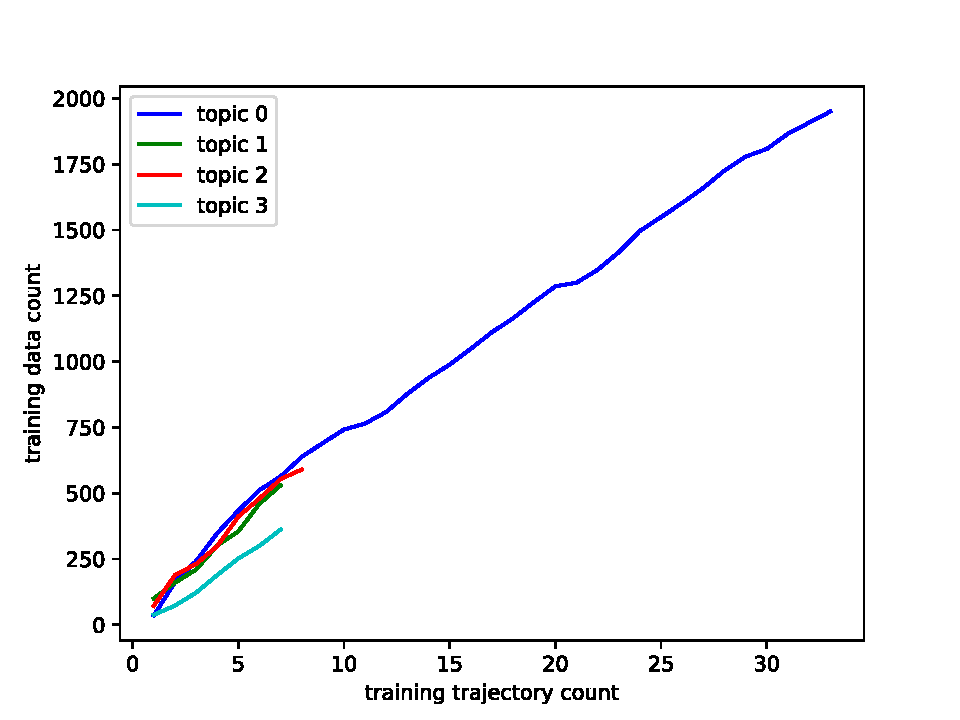
\includegraphics[width=\linewidth]{./img/gp/gp-ds.pdf}
    \caption{The training data count grows linearly with the training trajectory count.}
    \label{fig:gp-ds}
\end{figure}

Therefore, we have to maintain the $\mathbf{K}$ to a reasonable size and avoid computing $\mathbf{K}^{-1}$ too frequently to balance the computation overhead.
Some filtering and forgetting policies are applied here.
First, we only add the data that has enough change over the previously added data point.
Here $L1$ distance is used to measure the difference. 
Similar trajectory record between adjacent frames is often seen when the tracked object remains static in the scene or is too small to have a large change of size or velocity.
Second, we run hyper-parameter optimization upon the first batch of training data arrive; later we run the optimization with a longer interval.
Finally, after the training data has reached the maximal number, every time a new data point becomes available, it is added with a possibility of $p = 0.7$ and a random old data point is removed.
Moreover, once the $\mathbf{K}^{-1}$ is computed, the prediction only involves simple matrix multiplication.
We implement the algorithm on GPU to have fast matrix operation.

As the tracking continues, the covariance matrix $\mathbf{K}$ is maintained to a fixed size. 
We also keep a separate thread for computing $\mathbf{K}^{-1}$ and hyper-parameter optimization. 
The thread runs in the background without interrupting the tracker.
The above methods ensure the tracker still run in real time.
